\chapter{Vehículos automatizados}
\label{ape:carros}

El grupo AUTOPIA además del carro utilizado para las pruebas (Platero), poseen 4 vehículos más, que vamos a describir a continuación.

Dos camionetas eléctricas \textbf{Citroën Berlingo}, llamadas \textbf{Babieca} y \textbf{Rocinante}, que pueden verse en la figura \ref{fig:furgonetas}. Son impulsadas por un motor eléctrico de 15 Kw que puede alcanzar velocidades de hasta 90 Km/h; en pruebas de conducción automática se han alcanzado velocidades de 60 Km/h.

\begin{figure}[htb]
  \centering
  \includegraphics[width=0.5\textwidth]{figures/furgonetas.jpg}
  \caption{Babieca y Rocinante}
  \label{fig:furgonetas}
\end{figure}

Por otro lado, dos \textbf{Citroën C3 Pluriel}, uno de ellos descapotable, llamado \textbf{Clavideño} \cite{milanesCl}, y el otro llamado \textbf{Platero}, el cual utilizamos para la experimentación; ambos se muestran en la figura \ref{fig:c3s}

\begin{figure}[htb]
  \centering
  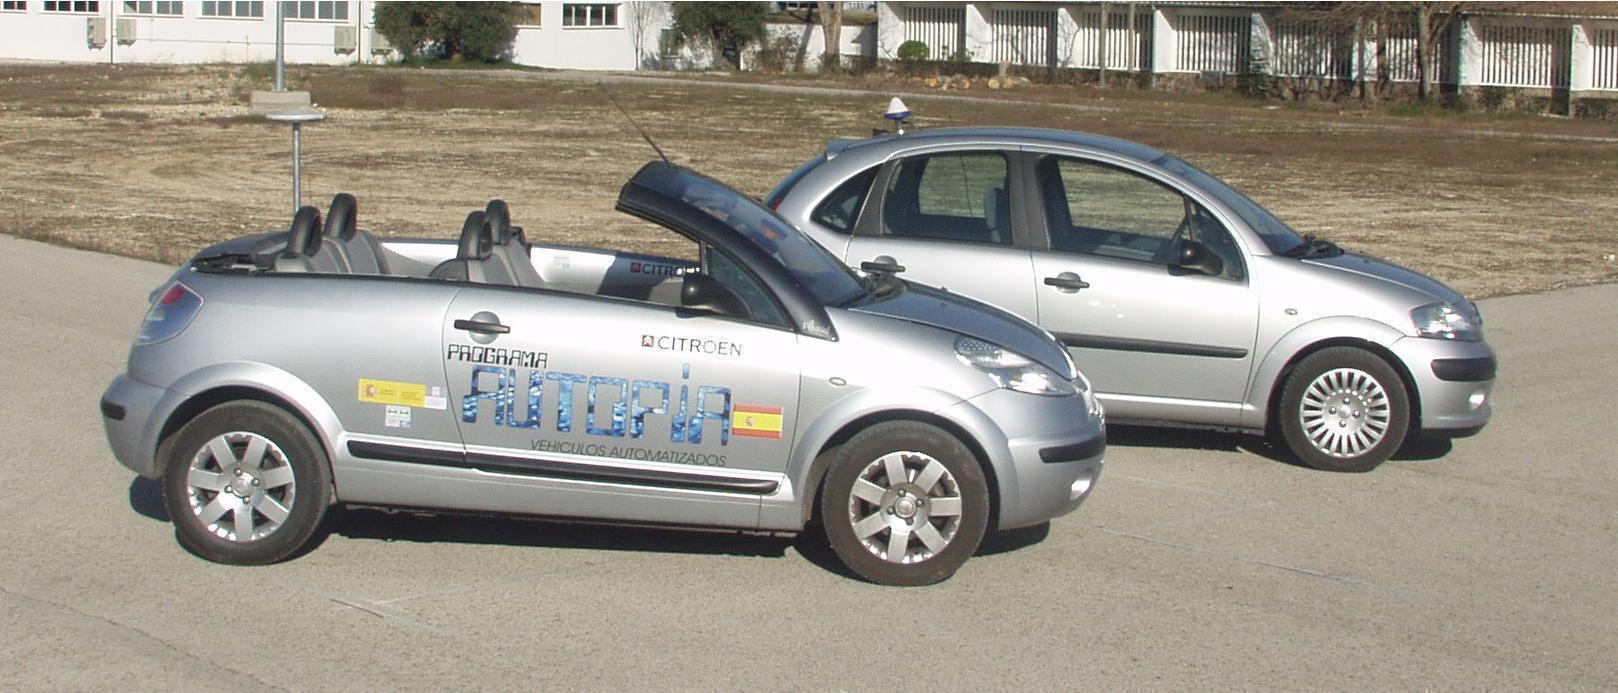
\includegraphics[width=0.5\textwidth]{figures/c3s.jpg}
  \caption{Clavideño y Platero}
  \label{fig:c3s}
\end{figure}

Finalmente, la última adquisición del grupo ha consistido en un prototipo de mini-autobús eléctrico para transporte público con el que se pretenden extrapolar las técnicas y resultados obtenidos a los sistemas públicos de transporte. Éste puede verse en la figura \ref{fig:molinero}.

\begin{figure}[htb]
  \centering
  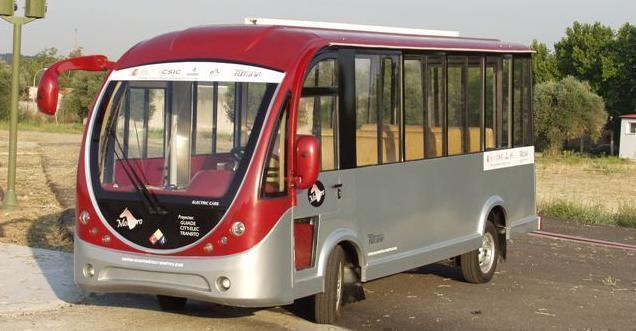
\includegraphics[width=0.5\textwidth]{figures/molinero.jpg}
  \caption{Molinero}
  \label{fig:molinero}
\end{figure}

\section{Sistema de navegación de Platero}
\label{ape:platero}

La información sensorial que el vehículo es capaz de leer de su entorno, está formada principalmente por un \gls{GPS}. Este, junto con la corrección diferencial suministrada por la estación base instalada en \gls{ZOCO} vía {WLAN}, permiten lecturas de posicionamiento de precisiones inferiores al centímetro.

En el caso de que, o bien el \gls{GPS} embarcado, o la comunicación con la estación base falle, una \gls{IMU} instalada junto a la palanca de cambios será capaz de dar la posición, usando para ello las aceleraciones frontales y laterales experimentadas por el automóvil, aunque con una precisión menor. Gracias a esto, el vehículo conocerá su posición en todo momento con una precisión centimétrica.

Por otra parte, la computadora del vehículo dispone de un mapa \gls{GPS} con la trayectoria a seguir, gracias a lo cual, y conociendo la posición actual se pueden inferir variables tales como el error lateral y angular respecto a la ruta deseada en un instante dado, así como la velocidad deseada en un determinado tramo de carretera     

\section{Sistema de aceleración y freno de Platero}
\label{ape:esquemas}


En lo que se refiere a la actuación necesaria para llevar a cabo un control de velocidad, se debe tener en cuenta únicamente el manejo de los pedales de acelerador y freno, dado que el vehículo utilizado (\textit{Platero}) dispone de su propio sistema de cambio de velocidades de la transmisión automático implementado por Citroën.

En lo que respecta al control del \textbf{acelerador}, se cortaron las dos señales de tensión que genera el acelerador y se conmutaron por otras generadas por el ordenador embarcado del vehículo.
 
Cuando un conmutador cambia de posición para activar el sistema de control automático, recibe una señal de una tarjeta externa de conexiones (modelo ADAM-3937) a la que se han derivado las señales analógicas de control provenientes de una tarjeta PCI 1720 \footnote{\url{ http://www.advantech.com.tw/products/PCI-1720/mod_1-2MLH37.aspx}}. Esta tarjeta se encarga de enviar las tensiones generadas por el controlador con el fin de regular la aceleración del vehículo, en la figura \ref{fig:esAce} se presenta el esquema correspondiente al sistema de aceleración.

\begin{figure}[htb]
\centering
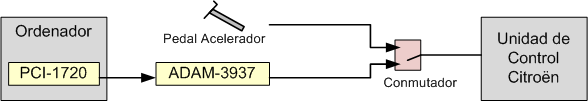
\includegraphics[width=0.8\textwidth]{figures/FuncionamientoAcelerador.png}
\caption{Esquema correspondiente al sistema de aceleración de Platero}
\label{fig:esAce}
\end{figure} 

Para el control del \textbf{freno}, se intervino la caja del \gls{ABS} con un sistema de actuación que consta de una válvula con una salida, conectada directamente al \gls{ABS} para respetar el circuito original. El sistema consta de dos entradas: la primera conectada al circuito inicial de freno, que permite su accionamiento convencional, y la segundo conectada a un sistema electro-hidráulico diseñado para el accionamiento automático del freno desde el ordenador embarcado. La válvula selectora se muestra en la figura \ref{fig:sysFre} (izquierda).

\begin{figure}[ht]
\begin{minipage}[b]{0.5\linewidth}
\centering
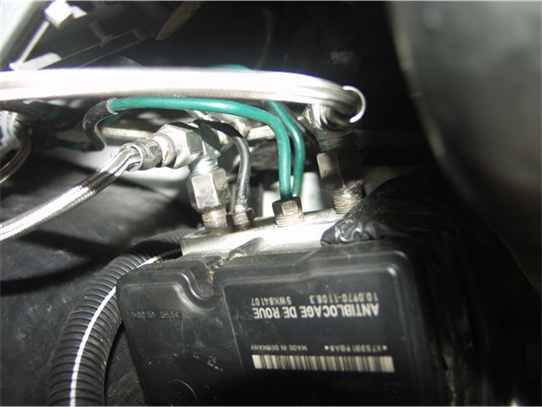
\includegraphics[width=0.8\linewidth]{figures/ValvulaFrenada.png}
\end{minipage}
\begin{minipage}[b]{0.5\linewidth}
\centering
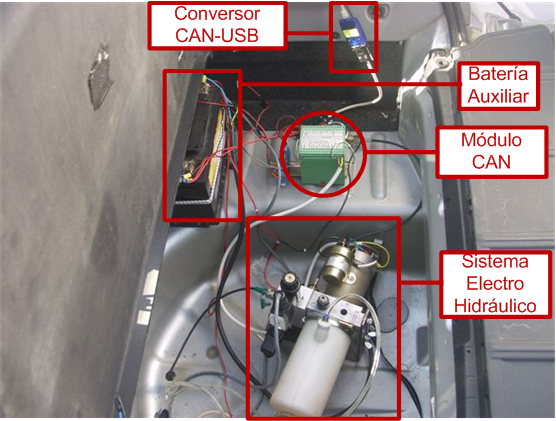
\includegraphics[width=0.8\linewidth]{figures/SistemaFrenada.png}
\end{minipage}
\caption{Válvula selectora entre sistema manual-automático (izquierda).Sistema de frenado electro hidráulico (derecha).}
\label{fig:sysFre}
\end{figure} 

El sistema electro-hidráulico esta formado, a su vez, por otras tres válvulas. Una \textit{limitadora} que impide superar la presión máxima, fijada experimentalmente en 100 bares, que se puede ejercer sobre el freno, una \textit{todo/nada} que permite el paso del líquido de freno y una \textit{proporcional} que regula su caudal. La válvula proporcional está controlada por el módulo \gls{CAN} con una salida analógica. Además, el dispositivo \gls{CAN} incluye una salida a relé para controlar la apertura y cierre de la válvula todo/nada. El módulo \gls{CAN} es alimentado por una batería auxiliar a la propia del vehículo. Las salidas son controladas a través del PC embarcado en el vehículo por medio de un conversor \gls{CAN}-USB. Todos los detalles de este sistema, pueden encontrarse en \cite{Milanes2010}. En la figura \ref{fig:sysFre} (derecha) se muestra una fotografía del sistema una vez montado en el vehículo. En la figura \ref{fig:esfreno} se presenta el esquema correspondiente al sistema de aceleración.

Ambos sistemas, para controlar el freno y el acelerador están implementados en el vehículo y pueden actuar conjunta o independientemente. Por otra parte, el funcionamiento de los sistemas de actuación no impide que un usuario pueda actuar sobre los pedales en caso de emergencia, o desactivarlos para realizar una conducción manual cuando lo desee. Con el sistema automático activado, el ordenador generará ordenes de control en el intervalo [0,1] que se traducirán en porcentaje de presión a aplicar sobre el correspondiente pedal.

\begin{figure}[htb]
\centering
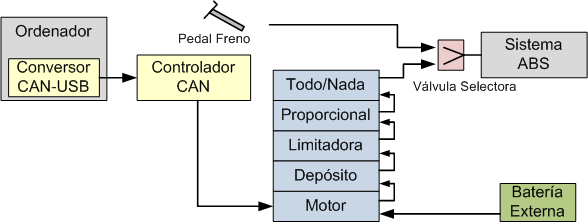
\includegraphics[width=0.8\textwidth]{figures/FuncionamientoFreno.png}
\caption{Esquema correspondiente al sistema de freno de Platero}
\label{fig:esfreno}
\end{figure}